To use the VMA306 sensor, we set the \textit{Trig} pin to \textbf{high} for at least \SI{10}{\micro s}, then the sensor send a burst of 8 x 40KHz pulses and set the \textit{echo} pin to \textbf{high}. When the burst comes back to the sensor (caused by the echo), the sensor set its \textit{echo} pin to \textbf{low} (illustrated on Figure \ref{fig:vma306}).

\begin{figure}[!ht]
 \centering
 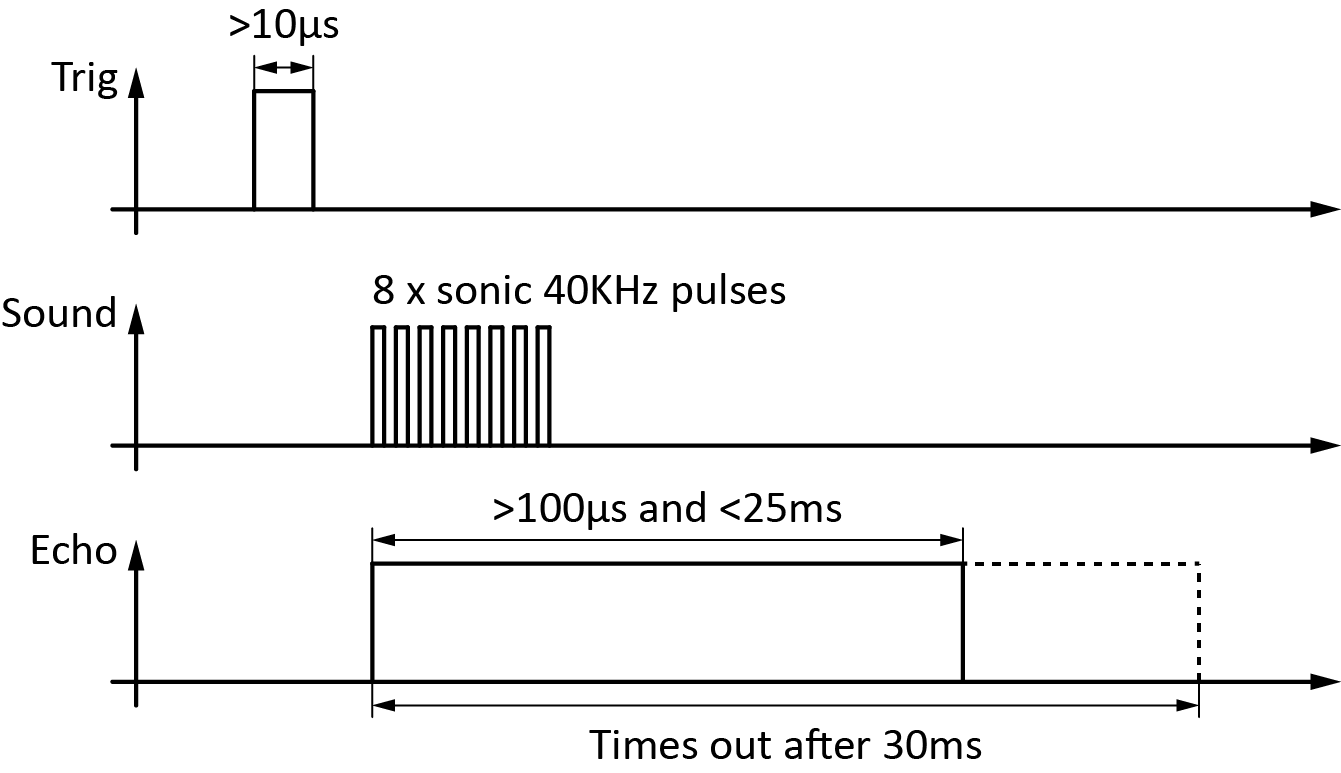
\includegraphics[width=.5\textwidth]{images/echo_vma}
 \caption{VMA306 sensor}
 \label{fig:vma306}
\end{figure}

Thus, the time during which the \textit{Echo} pin is \textbf{high} represent the time the sound traveled.
Let $t_{\text{up}}$ be the time of \textit{Echo} being \textbf{high} and $v_s = \SI{340}{m/s}$ the sound speed. The measured distance $d$ can be expressed as \[ d = v_s \times t_{\text{up}} \]



To avoid false detection each VMA306 send his pulse every 150ms and with a 50ms delay after previous one.
There are 3 VMA306 on the robot: one on the left, one on the front, one on  the right.

In the provided library, you can access to VMA306 data.
